\chapter{Guest Speaker David Swensen: The Yale Model and Long-Horizon Investing}

This chapter follows David Swensen's guest lecture in Robert J. Shiller's \emph{Financial Markets} course, curated here by LazyingArt LLC. The lecture opens with a live controversy rather than a formal model. Yale's endowment had become famous, then controversial, and Swensen uses that controversy to organize the whole hour. We begin with Barron's criticism of the ``Yale model,'' move backward to the portfolio world of 1985, then follow the lecture's central decomposition into asset allocation, market timing, and security selection. Only after that machinery is in place does Swensen return to the questions of diversification, liquidity, alternatives, and institutional performance.

\section{Opening challenge: the Yale model under criticism}

Shiller's introduction matters because it sets the stakes. He presents Swensen not only as Yale's endowment manager but as a serious financial innovator, someone associated with the early swap market, and he places Yale's long-run record in front of the audience before handing over the room. The subtext is clear: we are hearing from someone who has both built instruments and managed institutional capital.

Swensen begins in a different register. He jokes that the introduction would have sounded more flattering before the financial crisis. For many years the publicity around Yale's portfolio had been good. Then came Lehman, panic, and the inevitable backlash. A Barron's article from November 2008 had argued that colleges were suffering because the Yale model was too aggressive, too illiquid, and not truly diversified. Swensen's first move is to turn that criticism into the lecture's organizing question.

There is also a small but revealing rhetorical point here. Swensen notes the asymmetry in how people speak: when the portfolio succeeds it is the ``Yale model,'' and when it disappoints it becomes the ``Swensen approach.'' That joke does more than lighten the room. It marks the lecture's posture. He is not going to answer the criticism with branding. He is going to ask, from the ground up, what kind of portfolio a perpetual institution ought to hold.

So the lecture begins not with a defense of alternatives as such, and not with a narrow post-crisis performance argument. It begins with a structural question: what did the old endowment world look like, and what should a long-horizon investor do differently?

\section{1985 endowments and the two failed tests}

To answer that question Swensen goes back to 1985, when he arrived at Yale from Wall Street with no deep portfolio-management track record and did the sensible thing: he looked at what other endowed institutions were doing. The result, as he reports it, was remarkably uniform:
\begin{equation}
\left(w_{\text{US stocks}},\,w_{\text{US bonds+cash}},\,w_{\text{alternatives}}\right)
\approx (0.50,\,0.40,\,0.10).
\end{equation}
The lecture's diagnosis is that this conventional portfolio failed two basic tests. It failed the diversification test, and it failed the equity-orientation test.

On the first point Swensen invokes the finance theory associated with Tobin and Markowitz. Diversification is the famous ``free lunch'' of portfolio theory. He does not work through mean-variance geometry in the lecture, but the claim can be written in its standard form. If two portfolios have the same expected return, a better-diversified portfolio can carry lower variance,
\begin{equation}
E[R_p]=E[R_q], \qquad \sigma^2(R_p)<\sigma^2(R_q),
\end{equation}
and if two portfolios have the same variance, the better-diversified portfolio can carry higher expected return,
\begin{equation}
\sigma^2(R_p)=\sigma^2(R_q), \qquad E[R_p]>E[R_q].
\end{equation}
This is the abstract theory. Swensen's point is that the old endowment portfolios did not actually satisfy its spirit. A portfolio with half its assets in a single asset class is not meaningfully diversified, and a portfolio with ninety percent in domestic marketable securities is not drawing on a wide enough set of underlying return drivers.

His concrete example is interest rates. The lecture's language is intuitive: lower rates are good for bonds, and lower discount rates also raise the present value of future earnings streams, so they can be good for stocks as well. Since no validated board equation survives for this lecture, the clean way to sharpen that intuition is with the standard present-value formulas:
\begin{align}
P_{\text{bond}} &= \sum_{t=1}^{T}\frac{C_t}{(1+r)^t}+\frac{F}{(1+r)^T},\\
P_{\text{equity}} &= \sum_{t=1}^{\infty}\frac{CF_t}{(1+r)^t}.
\end{align}
The lecture does not insist that stocks and bonds always move together. The narrower point is that they can respond in the same direction to an important macro variable, so a portfolio made mostly of domestic stocks and domestic bonds is less diversified than it first appears.

The second failed test is equity orientation. Swensen's intuition is almost embarrassingly simple, and that is part of its force. Endowments have longer horizons than almost any other investors. Their job is to preserve purchasing power in perpetuity. That means they are natural bearers of equity risk. Yet the conventional endowment portfolio held about forty percent in bonds and cash, which Swensen treats as low expected return assets. On this view, the old structure was too timid for the institution it was meant to serve.

These are the two premises from which the Yale model grows: real diversification, and a meaningful commitment to equity-like risk for a perpetual investor.

\subsection{Question \& Answer}

\paragraph{Question.} If diversification was already standard finance theory, why were endowments still so badly structured?

\paragraph{Answer.} Swensen's answer is historical and institutional. The old endowment world had inherited a convention and learned to call it prudence. Once a portfolio shape becomes standard across peer institutions, it can survive by habit even when it is no longer defensible from first principles. The lecture's diagnosis is therefore not that diversification theory was unknown, but that portfolio practice had drifted away from the implications of the theory.

\section{Three tools of return}

Having reconstructed the old world, Swensen changes gears and introduces the framework that governs the rest of the lecture. There are, he says, three things we can do to affect portfolio returns.

First, we can decide what assets to own and in what long-run proportions. That is asset allocation.

Second, we can depart from those long-run weights because of a short-run valuation view. That is market timing.

Third, within an asset class, we can try to beat the market by overweighting some securities and underweighting others. That is security selection.

This is the lecture's main analytical hinge. Once the three levers are separated, the structure of the argument becomes much clearer. In note form we can summarize the decomposition as
\begin{equation}
R_p = R_{\text{policy}} + \alpha_{\text{timing}} + \alpha_{\text{selection}} - L,
\end{equation}
where \(R_{\text{policy}}\) is the return from the long-run policy portfolio, the \(\alpha\)'s are gains or losses from active deviations, and \(L\) denotes the leakages of active investing: fees, commissions, market impact, loads, taxes, and related costs.

The flow of the lecture can be summarized by the following editorial diagram:
\begin{figure}[h]
\centering
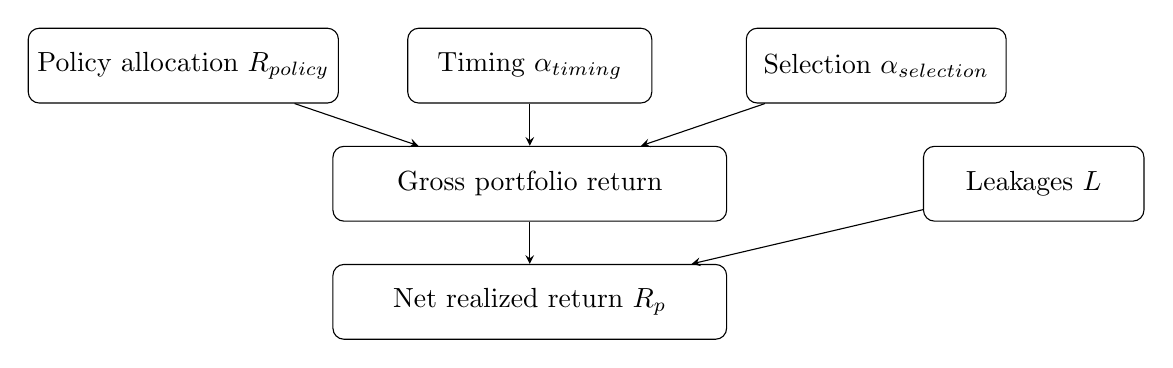
\begin{tikzpicture}[>=stealth]
\node[draw, rounded corners, minimum width=3.3cm, minimum height=0.95cm] (policy) at (0,1.5) {Policy allocation \(R_{\text{policy}}\)};
\node[draw, rounded corners, minimum width=3.1cm, minimum height=0.95cm] (timing) at (4.4,1.5) {Timing \(\alpha_{\text{timing}}\)};
\node[draw, rounded corners, minimum width=3.3cm, minimum height=0.95cm] (select) at (8.8,1.5) {Selection \(\alpha_{\text{selection}}\)};
\node[draw, rounded corners, minimum width=5.0cm, minimum height=0.95cm] (gross) at (4.4,0) {Gross portfolio return};
\node[draw, rounded corners, minimum width=2.8cm, minimum height=0.95cm] (leak) at (10.8,0) {Leakages \(L\)};
\node[draw, rounded corners, minimum width=5.0cm, minimum height=0.95cm] (net) at (4.4,-1.5) {Net realized return \(R_p\)};
\draw[->] (policy) -- (gross);
\draw[->] (timing) -- (gross);
\draw[->] (select) -- (gross);
\draw[->] (gross) -- (net);
\draw[->] (leak) -- (net);
\end{tikzpicture}
\end{figure}

The next step is especially important. Swensen says that asset allocation is ``far and away'' the most important tool, but he immediately warns us not to misunderstand that as a universal law of nature. If Yale put its entire endowment into Google stock, security selection would dominate. If Yale used the whole endowment to day-trade bond futures, market timing would dominate. These examples are deliberately absurd. Their purpose is to show that the dominance of asset allocation is behavioral rather than metaphysical.

Why, then, does asset allocation dominate in practice? Because real investors usually do something much more boring. They maintain a fairly stable long-run portfolio. They diversify within asset classes. They do not continually transform the entire endowment into one concentrated bet. Under those conditions the main determinant of realized return variation is the set of asset-class exposures themselves.

This is also how Swensen interprets the Ibbotson-style finding that more than ninety percent of the variability of institutional returns is attributable to asset allocation. Indeed, he pushes the point further. If market timing and security selection are zero-sum before costs and negative-sum after costs on average, then the policy portfolio explains more than one hundred percent of net returns:
\begin{equation}
\overline{\alpha_{\text{timing}}}+\overline{\alpha_{\text{selection}}}-\overline{L}<0.
\end{equation}
In other words, the active deviations do not merely fail to help on average; they subtract from what passive implementation of the policy portfolio would have produced.

\subsection{Question \& Answer}

\paragraph{Question.} Why can asset allocation be the dominant source of returns even though market timing and security selection also exist?

\paragraph{Answer.} Because the lecture's claim is conditional on sensible portfolio behavior. Once we assume that investors hold stable, diversified policy portfolios, the large-scale movements of asset classes dominate the return process. The cases in which timing or selection dominate are logically possible, but they are the pathological cases that Swensen uses precisely in order to set them aside.

\section{Long horizons, equity risk, and the trap of literalism}

Swensen now turns from framework to long-run evidence. Using Roger Ibbotson's historical data, he asks what would have happened to one dollar invested from the end of 1925 to 2009. The lecture is not interested in a tidy annualized abstraction. It wants the cumulative comparison:
\begin{align}
M_{\text{bills}} &= 21, &
M_{\text{inflation}} &= 12,\\
M_{\text{bonds}} &= 86, &
M_{\text{large stocks}} &= 2592,\\
M_{\text{small stocks}} &= 12226. &&
\end{align}
The immediate moral is that long-run investors are rewarded for accepting equity risk. Bills do not preserve much after inflation. Bonds are better, but still modest over many decades. Equities are in a different league entirely. So far the lecture's message is straightforward: a perpetual institution should carry meaningful exposure to risky productive assets.

But then Swensen performs one of the lecture's most important reversals. If the historical table is read too literally, it seems to imply something absurdly simple. If small stocks do best by such a large margin, why not put the whole endowment into small stocks? This is where the lecture's rhythm matters. Swensen lets the tempting inference appear before taking it apart.

\subsection{Question \& Answer}

\paragraph{Question.} If small stocks dominate the long-run data, why not put the whole endowment into small stocks?

\paragraph{Answer.} Because long-run arithmetic is not the whole problem. We must also ask whether the strategy is survivable. Swensen's chosen example is the Great Depression, and here the lecture slows down enough for us to work the arithmetic:
\begin{align}
W_{1929} &= W_0(1-0.54)=0.46W_0,\\
W_{1930} &= 0.46W_0(1-0.38)=0.2852W_0,\\
W_{1931} &= 0.2852W_0(1-0.50)=0.1426W_0,\\
W_{1932} &= 0.1426W_0(1-0.32)\approx 0.097W_0.
\end{align}
So the dollar at the peak becomes roughly ten cents at the trough. That is the worked mathematical example at the heart of the section, and it changes the problem completely. The question is no longer whether small stocks were best in the very long run. The question is whether an investor, however strong his stomach, can actually remain invested through such a collapse.

Swensen's answer is emphatically no. At some point dollars turning into dimes will overwhelm the abstract case for long-run expected return. This is why the lecture refuses the crude rule ``just own the thing with the highest historical multiple.'' Heavy equity exposure may be correct for a long-horizon investor, but undiversified concentration in one risky segment is not.

That is also why Swensen pauses to recall the cultural disgust for equities after the crash, the old language about stocks being ``insecurities.'' The point is not nostalgic. It is analytical. A strategy that cannot be held through the path of bad states is not a serious institutional policy. Diversification is what makes equity orientation liveable.

\section{Market timing and security selection as negative-sum behavior}

At this point the lecture pivots from long-run compounding to investor behavior. The second lever is market timing, and Swensen introduces it through Keynes. The relevant passage is memorable because it captures both the behavioral and the arithmetic problem: people who attempt large shifts sell too late, buy too late, do both too often, and pay heavy expenses in the process.

The lecture then supplies evidence. Morningstar compared time-weighted returns and dollar-weighted returns across seventeen categories of domestic-equity mutual funds. The distinction is central. Time-weighted returns describe the fund's own return path. Dollar-weighted returns tell us what investors actually experienced once their inflows and outflows are incorporated. Swensen's summary is strikingly simple:
\begin{equation}
R^{DW}<R^{TW}
\end{equation}
in every one of the seventeen categories. That is a remarkably clean empirical sign of perverse timing. Investors add money after good performance and pull money out after bad performance. They buy high and sell low.

The internet-fund example makes the same point with sharper narrative force. Swensen reports that the time-weighted return across the top internet funds over the six-year window around the bubble was about \(1.5\%\) per year. Yet investors allegedly put in roughly \$13.7 billion and lost roughly \$9.5 billion. The lecture's arithmetic at that moment is rough, but the logic is unmistakable. Investors were not steadily exposed through the whole period. They piled in near the top, then sold in disappointment after the collapse. Once again, the timing of the path mattered more than the headline statistic.

Nor do institutions escape. The October 1987 crash becomes the institutional analogue of the mutual-fund story. Stocks fell sharply, bonds rallied in a flight to safety, and institutions responded by selling stocks and buying bonds. Swensen's conclusion is blunt: both individuals and institutions have a recurring tendency to chase performance and thereby destroy returns.

Security selection is the third lever, and the lecture handles it with the simplest possible relative-market logic. If we buy the market inside an asset class, there is no active selection return:
\begin{equation}
\alpha_{\text{selection}}=0.
\end{equation}
If instead we overweight one stock and underweight another relative to the market, then someone else must hold the offsetting position. In aggregate, before costs,
\begin{equation}
\sum_i \alpha_i^{\text{selection}}=0.
\end{equation}
After commissions, market impact, management fees, consultant fees, loads, and taxes, it follows that
\begin{equation}
\sum_i\left(\alpha_i^{\text{selection}}-L_i\right)<0.
\end{equation}
Swensen applies a similar, though slightly looser, intuition to market timing in the aggregate. Someone's overweight relative to target must be another person's underweight, and once the cost of playing is included, timing too becomes negative-sum on average.

\subsection{Question \& Answer}

\paragraph{Question.} If active management is zero-sum before costs, why does the average active investor still lose?

\paragraph{Answer.} Because the lecture's actual object is not gross alpha but net alpha. Swensen's cited evidence gives only about a \(14\%\) chance of beating the market after fees and taxes. He then weakens even that figure. Many funds impose front-end loads, so the game is even more expensive than the published comparisons suggest. And survivorship bias flatters the winners by ignoring dead funds. Swensen's striking database numbers make the point concrete:
\begin{equation}
N_{\text{total}}=30{,}361,\qquad N_{\text{living}}=19{,}129,\qquad N_{\text{dead}}=11{,}232.
\end{equation}
A large fraction of funds disappear, mostly because they fail. The average investor therefore faces a game that is zero-sum before costs, negative-sum after costs, and statistically hard to win even before we correct the data for survivorship.

\section{Where active management matters}

Once the lecture has shown that active management is structurally costly, a new question arises. If active management is not attractive everywhere, where is it worth attempting? Swensen's answer is one of the lecture's most interesting practical refinements.

He proposes using dispersion as a proxy for opportunity. The exact quartile language in the transcript is a little noisy, so it is safest to speak generally of the spread between stronger and weaker managers in a given asset class. If a market is highly efficient, that spread should be tight. If it is less efficient, the spread should be wider:
\begin{align}
\Delta_{\text{bonds}} &\approx 0.5\% \text{ per year},\\
\Delta_{\text{large cap}} &\approx 2.0\% \text{ per year},\\
\Delta_{\text{foreign}} &\approx 4.0\% \text{ per year},\\
\Delta_{\text{absolute return}} &\approx 7.1\% \text{ per year},\\
\Delta_{\text{real estate}} &\approx 3.0\% \text{ per year},\\
\Delta_{\text{LBO}} &\approx 13.7\% \text{ per year},\\
\Delta_{\text{VC}} &\approx 43.2\% \text{ per year}.
\end{align}

The lecture's interpretation is not abstractly efficient-market in tone. It is operational. Bonds are ``just math''---coupons, principal, probabilities of default. They are easier to analyze, so the scope for persistent skill is smaller. That is why managers in those markets tend to be packed close together. The safest thing for a manager to do in such an environment is often to hug the benchmark.

At the other end are private markets, especially venture capital. There may not even be a benchmark that can be mechanically replicated. The assets are idiosyncratic, the enterprises are private, and manager skill can matter much more. This is why Swensen's argument for alternatives is never simply ``private markets are good.'' It is instead: if active management is costly everywhere, then we should spend our active effort where the opportunity set is widest.

The audience questions sharpen this point. Swensen is asked whether the growth of hedge funds and private equity has made those markets too efficient to bother with. His answer is nuanced. Fees and leakages have unquestionably grown; that makes the negative-sum problem worse. But he does not think dispersion has collapsed. So long as the spread between the best and worst managers remains large, the activity remains potentially worthwhile for an institution able to identify superior managers.

\section{Returning to Barron's: diversification, alternatives, and the institutional coda}

Only now does Swensen return to Barron's. On diversification, he grants a narrow point: in a panic, diversification can appear to fail. Investors compress the world into two bins, risk and safety. Risky assets are sold together, and U.S. Treasuries become the unique refuge. In that window, the only thing that looks like protection is ownership of the asset everyone is running toward.

But Swensen insists that this is the wrong horizon on which to judge portfolio design. To hold a very large Treasury position all the time is to pay a large opportunity cost year after year. The panic window may last six months or a year; the cost of defensive underinvestment can last decades. That is why he brings in Japan. If one had wanted an equity-oriented portfolio but held only domestic Japanese equities, then from 1989 to 2009 one would have lived through a roughly seventy-three percent decline:
\begin{equation}
\text{Nikkei}_{1989}\approx 38{,}000,\qquad \text{Nikkei}_{2009}\approx 10{,}500,
\end{equation}
so that
\begin{equation}
1-\frac{10{,}500}{38{,}000}\approx 0.724 \approx 73\%.
\end{equation}
The lesson is exact and limited. Diversification may disappoint in a panic, but concentration can destroy long-run purchasing power.

On the charge of overemphasizing alternatives, Swensen shifts from principle to record. Over the ten years ending June 30, 2010, Yale's returns in several alternative sectors were stronger than in domestic public equities:
\begin{align}
R_{\text{domestic eq}} &\approx -0.7\%\ \text{per year},&
R_{\text{bonds}} &\approx 5.9\%\ \text{per year},\\
R_{\text{private eq}} &\approx 6.2\%\ \text{per year},&
R_{\text{real estate}} &\approx 6.9\%\ \text{per year},\\
R_{\text{absolute return}} &\approx 11.1\%\ \text{per year},&
R_{\text{timber}} &\approx 12.1\%\ \text{per year},\\
R_{\text{oil\&gas}} &\approx 24.7\%\ \text{per year}.&&
\end{align}
He then broadens the performance comparison to Yale as a whole. The lecture cites approximately \(8.9\%\) per year over ten years versus an average university figure near \(4.0\%\), and approximately \(13.1\%\) over twenty years versus a university average near \(8.8\%\). The tone at this point is understandably firm. Barron's, he argues, had looked at too short a window.

The final audience questions turn this defense into practical advice. Swensen says Yale's job differs from a hedge fund manager's in an important way: Yale sits one layer above direct security selection. Its central task is to find and structure relationships with excellent managers. That is why the principal-agent problem becomes so important. Yale must induce agents to act in the university's interest.

He also distinguishes institutions like Yale from ordinary investors on taxes and resources. Yale does not pay taxes; individuals do. Yale can devote a professional staff to manager selection; most individuals cannot. This is why, when asked what ordinary investors should do, Swensen does not tell them to imitate the full Yale model. He tells them to choose a sensible policy allocation and implement it with low-cost index funds.

\subsection{Question \& Answer}

\paragraph{Question.} If diversification fails during panics, why should a long-term investor still insist on it?

\paragraph{Answer.} Because the long-term investor's problem is not to maximize comfort in a panic; it is to preserve purchasing power across decades without being ruined by concentration. Panic behavior and long-run portfolio design are not the same question. A portfolio that looks brilliant only in crisis and costly the rest of the time is not obviously well designed. Swensen's answer is that the right comparison must include both the opportunity cost of too much safety and the catastrophic risk of country or asset-class concentration.

That same logic reappears when Swensen answers a later question about whether stocks are currently expensive. His first response is not a market forecast. It is that the valuation question matters less in a well-diversified portfolio with disciplined rebalancing. Once we have target weights \(w_i^{*}\), rebalancing pulls realized weights back toward policy:
\begin{equation}
w_i \to w_i^{*}.
\end{equation}
The arithmetic is plain. If an asset underperforms and drifts below target, we buy it back up to target; if it outperforms and drifts above target, we trim it back down. The lecture's later numerical guidance is therefore practical and memorable: a diversified portfolio may have something like a \(5\%\) to \(10\%\) minimum position and a \(25\%\) to \(30\%\) maximum position in any one asset class. Within such a structure, rebalancing quietly accomplishes much of what investors wrongly try to do with dramatic market timing.

Swensen is also asked about technology exposure. His answer is consistent with the earlier dispersion argument. Yale has a longstanding venture-capital commitment, and it also uses managers who specialize in technology and biotechnology because those sectors can be less efficiently priced than more mature public-equity segments. So even here the lecture's general rule holds: do not speculate because a sector is fashionable, but do recognize that some markets may offer more room for skilled selection than others.

The last important caution concerns risk measurement. Swensen is explicitly skeptical of simple Sharpe-ratio comparisons across institutional portfolios:
\begin{equation}
\text{Sharpe}=\frac{E[R_p-R_f]}{\sigma(R_p)}.
\end{equation}
He does not reject the formula; he rejects the casual use of the denominator. Public markets are marked continuously and exhibit large measured standard deviations. Illiquid assets are appraised infrequently, and appraisal smoothing mechanically lowers reported volatility. So when we compare a marketable-securities portfolio to a portfolio heavy in illiquid assets, we are not necessarily comparing like with like. In his terms, this is an apples-and-oranges problem.

The lecture ends with one final sharp contrast. For those with extraordinary resources and genuine access to superior managers, aggressive active management may make sense. For everyone else, the middle ground is the most dangerous place to stand. One ends up paying high fees for mediocre active results. That is why Swensen's practical advice for most investors is a disciplined passive policy, not a watered-down imitation of institutional complexity.

\section{Summary}

Swensen's lecture begins as a defense of the Yale model, but by the end it has become something more general: a theory of how a long-horizon institution should think. The first principle is that endowments ought to be equity oriented because their horizon is long and their mission is to preserve purchasing power in perpetuity. The second is that real diversification is broader than a conventional mix of domestic stocks and bonds. The third is that once we separate asset allocation from market timing and security selection, we see why active behavior so often subtracts from rather than adds to returns.

The lecture never says that all alternatives are good, or that diversification is magic in every state of the world. Its claim is more precise. Diversification can fail in a panic and still be indispensable over decades. Active management can be negative-sum in the aggregate and still be worth pursuing in unusually wide-dispersion markets for institutions with exceptional resources. And for most investors, the right response to all this is not complexity for its own sake, but a sensible policy portfolio, disciplined rebalancing, and a refusal to confuse excitement with investment intelligence.